\documentclass[crop,tikz,convert={outext=.svg,command=\unexpanded{pdf2svg \infile\space\outfile}},multi=false]{standalone}
\usepackage{tikz}
\usepackage{bm}
\usetikzlibrary{positioning}

\begin{document}

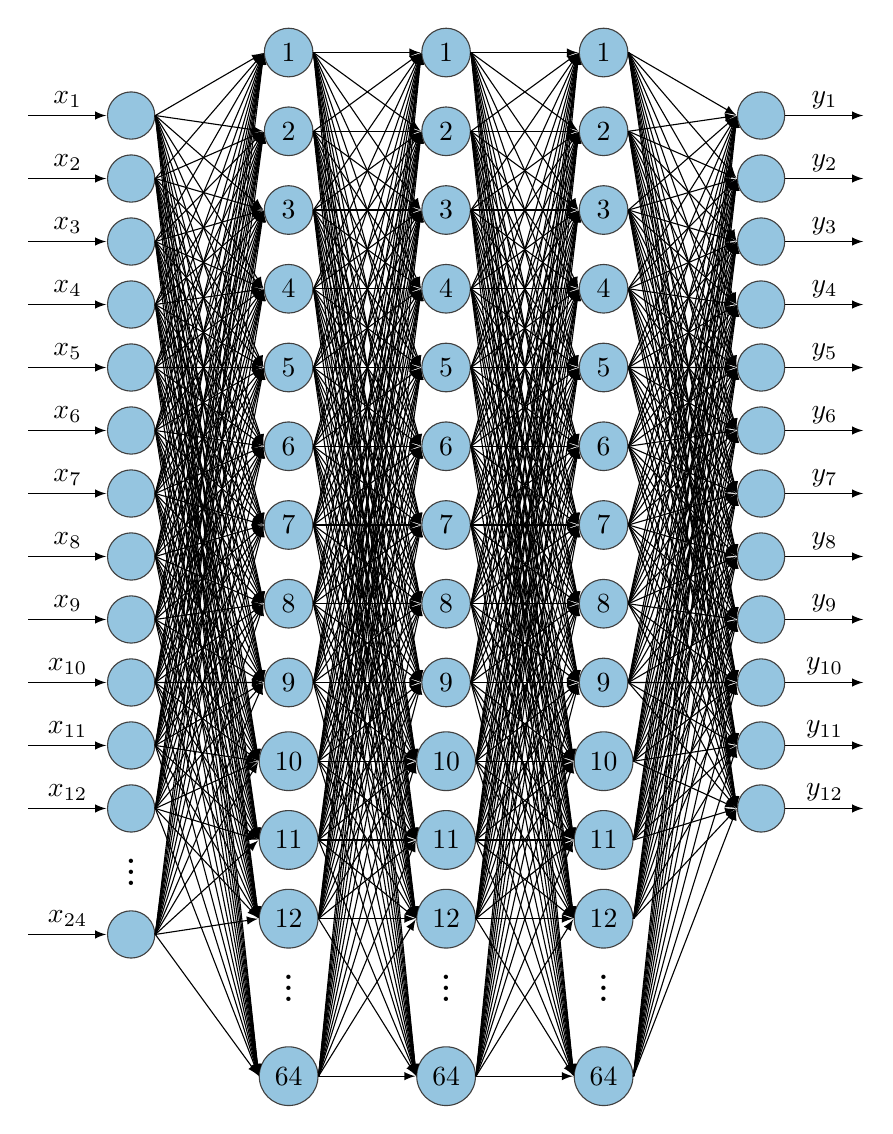
\begin{tikzpicture}[node distance=0.6cm and 0.6cm]
    \tikzset{every path/.style={shorten >=0.1mm}}
\definecolor{Masch_light}{RGB}{149,197,224}
% Eingabeschicht (24 Neuronen)
\foreach \i in {1,...,12} {
    \node[circle, draw=black!75,fill=Masch_light, minimum size=0.6cm] (input\i) at (0,-\i*0.8-1) {};
}
\node[circle, draw=black!75,fill=Masch_light, minimum size=0.6cm] (input13) at (0,-14*0.8-1) {};
\node[align=center] ()[below=-0cm of input12] {$\bm{\vdots}$};
% Erste versteckte Schicht (8 Neuronen)
\foreach \i in {1,...,12} {
    \node[circle, draw=black!75,fill=Masch_light, minimum size=0.6cm] (hiddenA\i) at (2,-\i*1) {\i};
}
\node[align=center] ()[below=-0cm of hiddenA12] {$\bm{\vdots}$};
\node[circle, draw=black!75,fill=Masch_light, minimum size=0.6cm] (hiddenA13) at (2,-14*1) {64};

% Zweite versteckte Schicht (8 Neuronen)
\foreach \i in {1,...,12} {
    \node[circle, draw=black!75,fill=Masch_light, minimum size=0.6cm] (hiddenB\i) at (4,-\i*1) {\i};
}
\node[align=center] ()[below=-0cm of hiddenB12] {$\bm{\vdots}$};
\node[circle, draw=black!75,fill=Masch_light, minimum size=0.6cm] (hiddenB13) at (4,-14*1) {64};

% Dritte versteckte Schicht (8 Neuronen)
\foreach \i in {1,...,12} {
    \node[circle, draw=black!75,fill=Masch_light, minimum size=0.6cm] (hiddenC\i) at (6,-\i*1) {\i};
}
\node[align=center] ()[below=-0cm of hiddenC12] {$\bm{\vdots}$};
\node[circle, draw=black!75,fill=Masch_light, minimum size=0.6cm] (hiddenC13) at (6,-14*1) {64};

% Ausgabeschicht (12 Neuronen)
\foreach \i in {1,...,12} {
    \node[circle, draw=black!75,fill=Masch_light, minimum size=0.6cm] (output\i) at (8,-\i*0.8-1) {};
}

% Verbindungen: Eingabe -> Hidden A
\foreach \i in {1,...,13} {
    \foreach \j in {1,...,13} {
        \draw[-latex] (input\i.east) -- (hiddenA\j.west);     
    }
}

% Verbindungen: Hidden A -> Hidden B
\foreach \i in {1,...,13} {
    \foreach \j in {1,...,13} {
        \draw[-latex] (hiddenA\i.east) -- (hiddenB\j.west);
    }
}

% Verbindungen: Hidden B -> Hidden C
\foreach \i in {1,...,13} {
    \foreach \j in {1,...,13} {
        \draw[-latex] (hiddenB\i.east) -- (hiddenC\j.west);
    }
}

% Verbindungen: Hidden C -> Ausgabe
\foreach \i in {1,...,13} {
    \foreach \j in {1,...,12} {
        \draw[-latex] (hiddenC\i.east) -- (output\j.west);
    }
}

% Eingangs x
\foreach \i in {1,...,12} {
    \draw[-latex] ([xshift=-1cm]input\i.west) -- node[yshift=0.2cm] {$x_{\i}$}(input\i.west);
}
\draw[-latex] ([xshift=-1cm]input13.west) -- node[yshift=0.2cm] {$x_{24}$}(input13.west);

% Ausgangs y
\foreach \i in {1,...,12} {
        \draw[-latex] (output\i.east) -- node[yshift=0.2cm] {$y_{\i}$}([xshift=1cm]output\i.east);
}

\end{tikzpicture}

\end{document}
